\documentclass[11pt, a4paper]{article}

\usepackage[affil-it]{authblk}
\usepackage{etoolbox}
\usepackage{lmodern}
\usepackage{titlesec}
\usepackage{float}
\usepackage{amsfonts}
\usepackage{hyperref}
\usepackage{listings}
\usepackage{color}
\usepackage{graphicx}
\usepackage{subcaption}
\usepackage{amsmath}
\usepackage{relsize}
\usepackage[a4paper, margin=1in]{geometry}

\makeatletter
\patchcmd{\@maketitle}{\LARGE \@title}{\fontsize{20}{19.2}\selectfont\@title}{}{}
\makeatother

\renewcommand\Authfont{\fontsize{16}{14.4}\selectfont}
\renewcommand\Affilfont{\fontsize{12}{10.8}\itshape}

\title{\textbf{PH 810: Project}}
\author{Pavan R Hebbar - 130010046}

\definecolor{codegreen}{rgb}{0,0.6,0}
\definecolor{codegray}{rgb}{0.5,0.5,0.5}
\definecolor{codepurple}{rgb}{0.58,0,0.82}
\definecolor{backcolour}{rgb}{0.95,0.95,0.92}
 
\lstdefinestyle{mystyle}{
    backgroundcolor=\color{backcolour},   
    commentstyle=\color{codegreen},
    keywordstyle=\color{magenta},
    numberstyle=\tiny\color{codegray},
    stringstyle=\color{codepurple},
    basicstyle=\footnotesize,
    breakatwhitespace=false,         
    breaklines=true,                 
    captionpos=b,                    
    keepspaces=true,                 
    numbers=left,                    
    numbersep=5pt,                  
    showspaces=false,                
    showstringspaces=false,
    showtabs=false,                  
    tabsize=2
}
\lstset{style=mystyle}

\begin{document}
\maketitle
\newpage
\tableofcontents
\newpage
\section{Introduction}:
This project deals with the three body decay of $\Lambda^0$ particle to one neutron and two $\gamma$ particles. All the 
analysis has been done for two dimensions.

\section{Description of Classes used}:
A main class \emph{Particles} is defined which provides the basic functions to declare a particle and set its mass and 
momentum and also to know them. Momentum can be set using its vector components or by specifying its direction and the 
magnitude. A function is also included for getting to know the energy of the particle. Since this problem deals with two
sequential two body decays, a function has been included for knowing the momentum of the two decay particles given their mass.

Class \emph{Lambda} inherits the class \emph{Particles} but sets the default value of mass as $1115.683 MeV/c^2$ when constructed. Same is the 
case with classes \emph{Neutron}, \emph{Pion} and \emph{Gamma} which set the corresponding default vales of mass. The class 
\emph{Gamma} also includes function to randomize the detected energy within the given relative error.

\section{Decription of the code}:
First, $10000$ lambda particles are created using function \emph{gen\_lambda} is defined to generate a given number of lambda particles. The lambda particles are
generated with a exponential $p_T$ distribution with $\tau = 1 GeV/c^2$ and a gaussian psuedorapidity distribution with mean 0
and sigma of 1. 

Each of the lambda particle is then decayed to a neutron and a pion and the pion is further decayed into two gamma particles.
The energy of these gamma particles are then randomized within a relative error of $5\%$.

Using the decay products we reconstruct the mass of lambda particle using the function \emph{get\_lmass}. For the analysis of the
results functions are inluded to get the invariant masses and plot the Dalitz plot

\section{Results}:
The Dalitz plots are given below:
\begin{figure}[H]
 \centering
 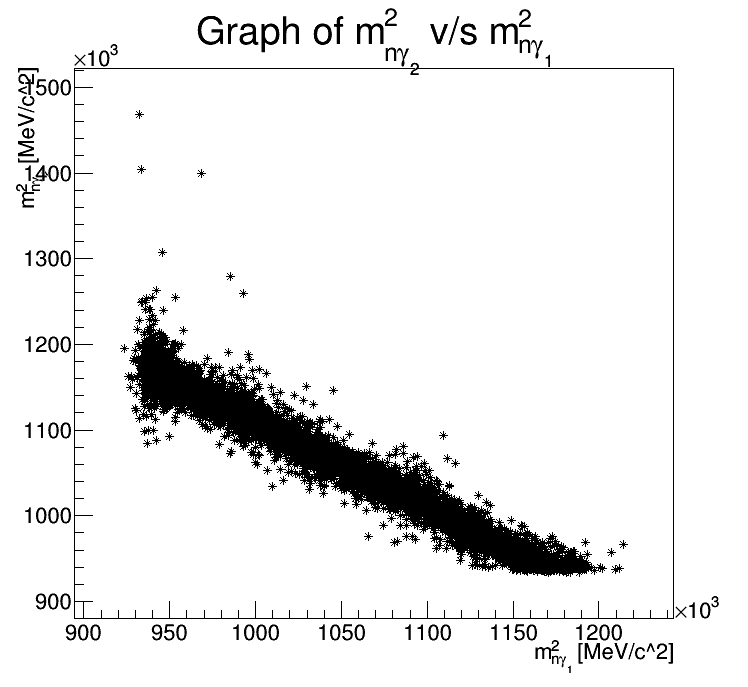
\includegraphics[width = 0.9\textwidth]{ng2_ng1.png}
\end{figure}

\begin{figure}[H]
 \centering
 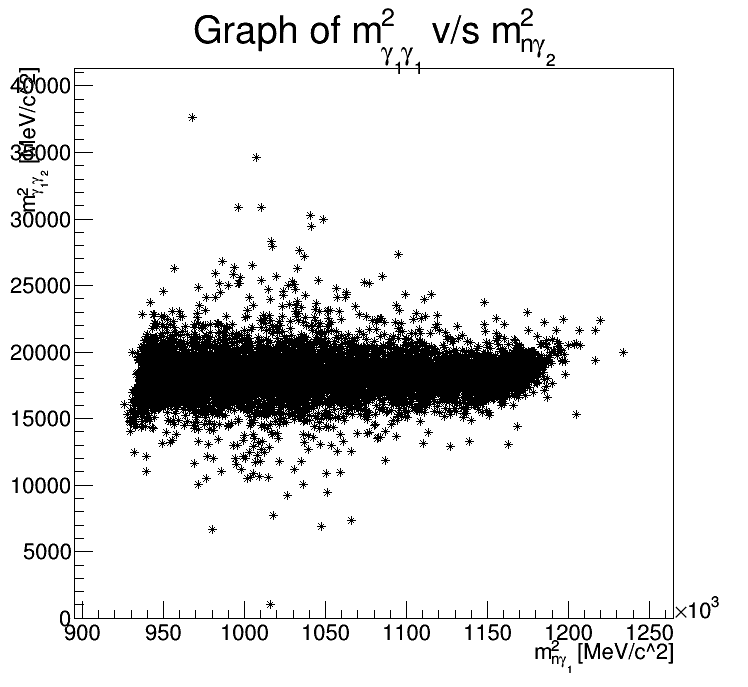
\includegraphics[width = 0.9\textwidth]{g1g2_ng2.png}
\end{figure}

Note that these plots are for cases when we know the neutrons and photons corresponding to a given lambda particle decay.
An attempt was made to calculate the invariant masses of all possible combinations and plot them. But the result hasn't been 
included as they weren't satisfactory.

Since the energy of photons were randomized it was observed that the reconstructed mass of lambda particle changed slightly 
each time the code was executed. But the result was very close to the actual mass of $1115.6$ within 4 significant digits.

\section{Conclusion}:
We see that the Dalitz plot of $m_{n\gamma_2}$ v/s $m_{n\gamma_1}$ is a straight line within error bounds. In fact, we can
see from calculations that $m_{n\gamma_2} ^2 + m_{n\gamma_1} ^2 = m_{\lambda ^0}^2 + m_n ^2 - m_{\pi} ^2$ and the result 
agrees with this. 

The plot of  $m_{\gamma_1 \gamma_2}$ v/s $m_{n\gamma_2}$ is roughly a constant equal to $m_{\pi} ^2$






\end{document}

